\begin{frame}
    \frametitle{GPU Computing}
    \framesubtitle{Introduction}

    \begin{columns}
        \begin{column}{0.5\textwidth}
            \begin{itemize}
                \item \emph{``Using a GPU (Graphic Processing Unit) together with
                      a CPU to accelerate scientific calculation operations
                      or general purpose calculation''}
            \end{itemize}
        \end{column}
        \begin{column}{0.5\textwidth}
             \begin{figure}
                 \centering
                 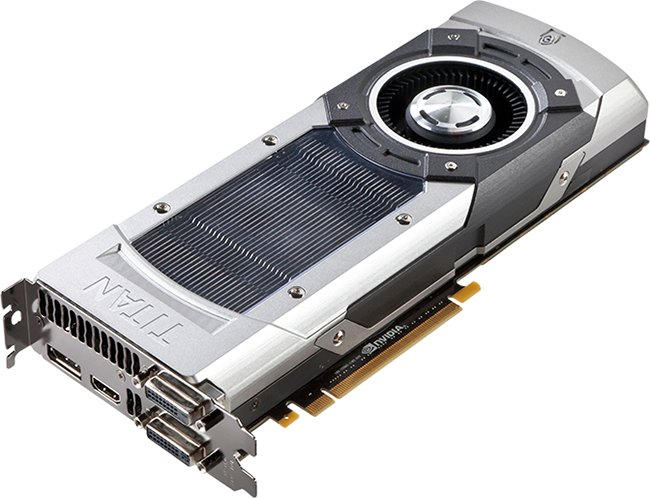
\includegraphics[width=0.8\textwidth]{img/titan}
                 \caption{NVIDIA\textsuperscript{\textregistered} GTX Titan}
                 \label{fig:titan}
             \end{figure}
        \end{column}
    \end{columns}
\end{frame}

\begin{frame}
    \frametitle{GPU Computing}
    \framesubtitle{Features}

    \begin{itemize}
        \item CPU,
        \begin{itemize}
            \item Designed to have a good \blue{performance}
                  in parallel and non-parallel scenarios.
            \item Minimizes the \blue{latency} experimented by a thread
                  (large cache memory)
        \end{itemize}
        \item GPU,
            \begin{itemize}
            \item Designed to perform highly parallel work.
            \item Maximizes the \blue{throughput} of all the threads.
            \end{itemize}
    \end{itemize}

    \begin{footnotesize}
        \begin{columns}
            \begin{column}{0.35\textwidth}
            \begin{block}{Performance}
                Capacity of perform individual instructions in a certain time.
            \end{block}
            \end{column}
            \begin{column}{0.3\textwidth}
            \begin{block}{Latency}
                Measure of time delay experienced in a system.
            \end{block}
            \end{column}
            \begin{column}{0.3\textwidth}
            \begin{block}{Throughput}
                Capacity of perform a whole task in a certain time.
            \end{block}
            \end{column}
        \end{columns}
    \end{footnotesize}

    %\begin{description}
    %    \item[Performance]
    %            Capacity of perform individual instructions in a certain time.
    %    \item[Throughput]
    %            Capacity of perform a whole task in a certain time.
    %    \item[Latency]
    %            Measure of time delay experienced in a system.
    %    \item[Granularity]
    %            Break down a system into small parts.(Coarse and Fine)
    %\end{description}
\end{frame}

\begin{frame}
    \frametitle{GPU Computing}
    \framesubtitle{Architecture}

    \begin{columns}
        \begin{column}{0.5\textwidth}
            \begin{block}{Task parallelism}
                Each processor perform a different task.
            \end{block}
            \begin{block}{Data parallelism}
                Each processor perform the same task, but not on the same data set.
            \end{block}
        \end{column}
        \begin{column}{0.5\textwidth}
             \begin{figure}
                 \centering
                 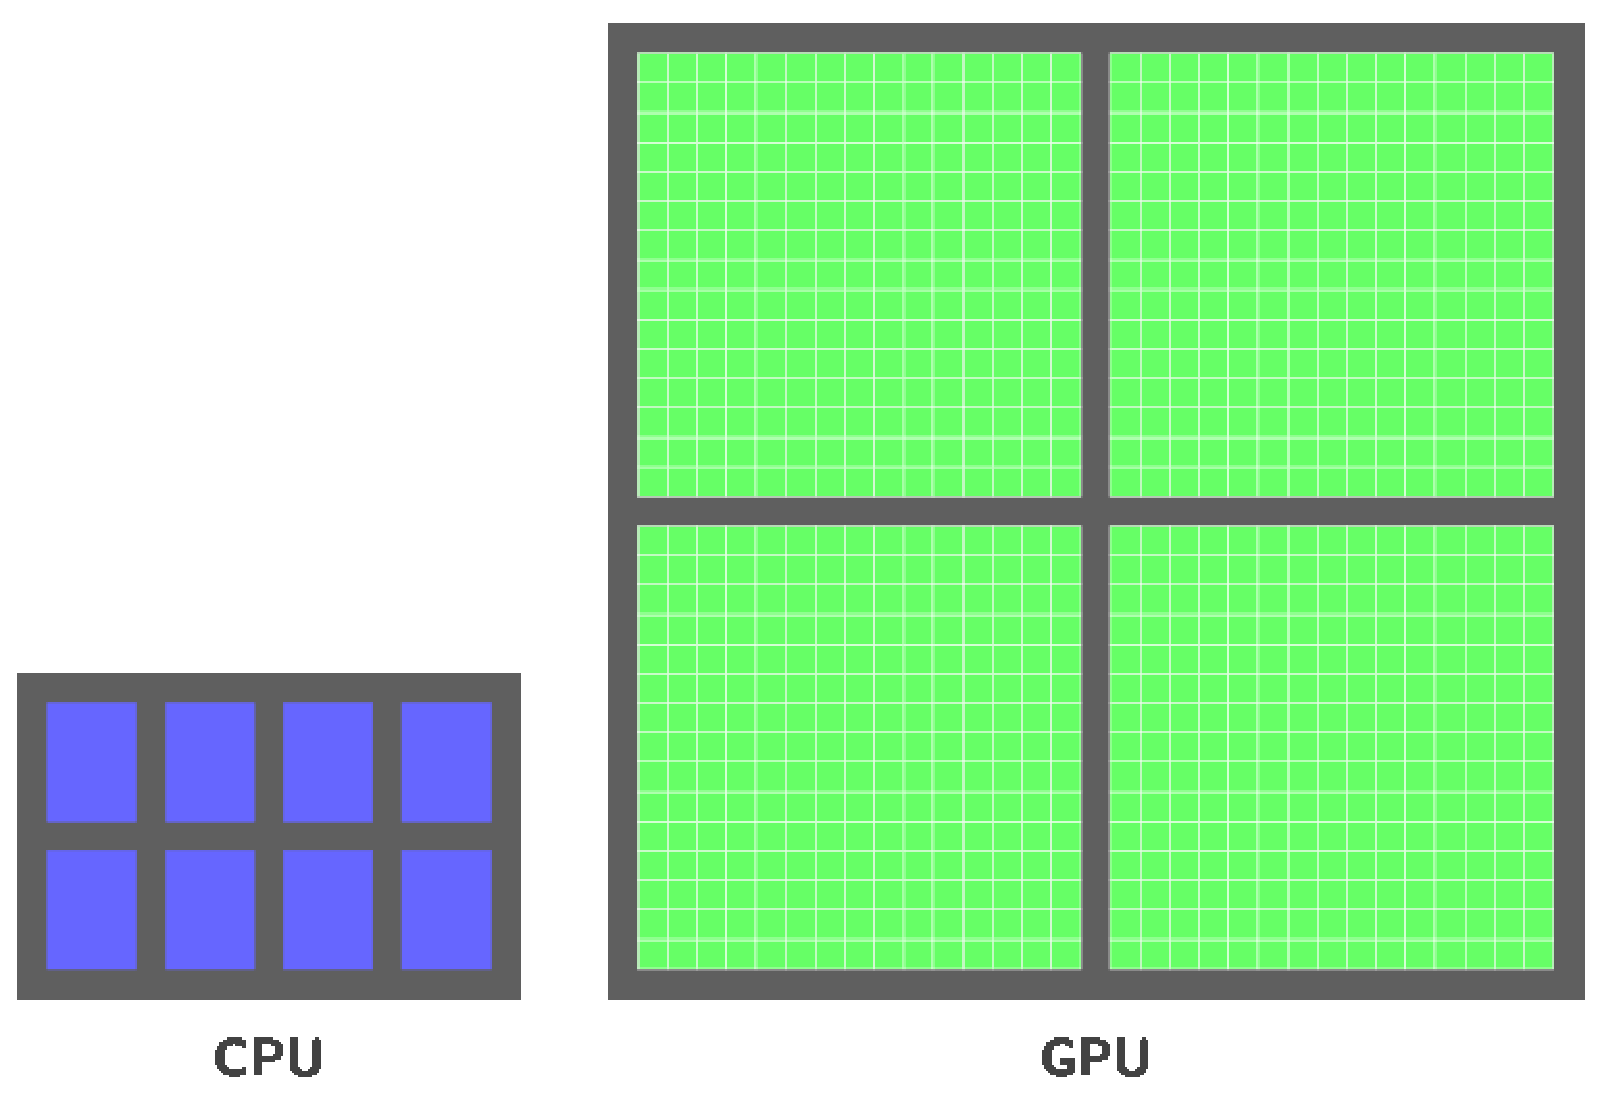
\includegraphics[width=0.8\textwidth]{img/cpu_gpu}
                 \caption{GPU and CPU core scheme}
                 \label{fig:titan}
             \end{figure}
        \end{column}
    \end{columns}
\end{frame}

\begin{frame}
    \frametitle{GPU Computing}
    \framesubtitle{Functionality}

    \begin{columns}
        \begin{column}{0.5\textwidth}
            \begin{figure}
                \captionsetup{singlelinecheck=off}
                \centering
                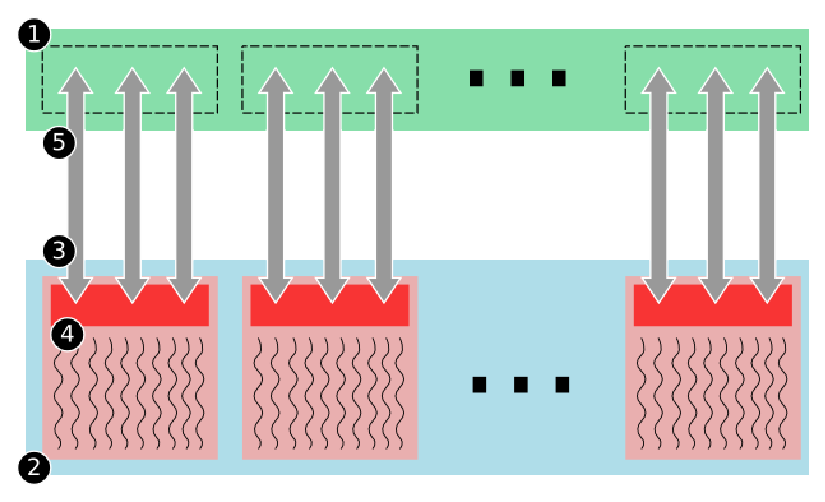
\includegraphics[width=0.9\textwidth]{img/cuda-strategy}
                \label{fig:estrategia}
                \caption{CUDA Programming strategy}
            \end{figure}
        \end{column}
        \begin{column}{0.5\textwidth}
             \begin{enumerate}
                 \item CPU memory allocation,
                 \item \dgreen{GPU} memory allocation,
                 \item Data copying,  CPU $\rightarrow$ \dgreen{GPU},
                 \item Task execution on the data,
                 \item Data copying, \dgreen{GPU} $\rightarrow$ CPU,
             \end{enumerate}
        \end{column}
    \end{columns}
\end{frame}

